\chapter{Implementacija i korisničko sučelje}
		
		
		\section{Korištene tehnologije i alati}
		
		
			Komunikacija u timu ostvarena je korištenjem aplikacije WhatsApp \footnote{\url{https://www.whatsapp.com/}}. Kao sustav za upravljanje izvornim kodom korišten je Git \footnote{\url{https://git-scm.com/}}, a izvorni kod projekta dostupan je na Github \footnote{\url{https://github.com/}} web platformi . Za izradu dokumentacije korištena je distribucija markup jezika LaTeX MiKTeX \footnote{\url{https://miktex.org/}}  u kombinaciji s TeXstudio \footnote{\url{https://www.texstudio.org/}} radnom okolinom.
				
			Za izradu aplikacije koristila su se dva razvojna okruženja, Visual Studio Code\footnote{\url{https://code.visualstudio.com/}} za frontend i JetBrains IntelliJ IDEA \footnote{\url{https://www.jetbrains.com/idea/}} za backend. Visual Studio Code je radna okolina koju razvija i održava Microsoft, vrlo je fleksibilna te omogućava razvoj u širokom spektru jezika i tehnologija. JetBrains IntelliJ IDEA je razvojno okruženje specifično dizajnirano za rad s programskim jezikom Java, održava je tvrtka JetBrains koja je poznata po proizvodnji razvojnih okolina.
			
			Za izradu backenda korišten je programski jezik Java\footnote{\url{https://www.java.com/en/}} i radni okvir Spring \footnote{\url{https://spring.io/}}. Spring je radni okvir koji nudi gotova rješenja za mnoge često potrebne funkcionalnosti programskih sustava, time programerima omogućuje jednostavniji, brži i sigurniji razvoj aplikacija. 
			
			Za izradu frontenda korišten je programski jezik JavaScript\footnote{\url{https://developer.mozilla.org/en-US/docs/Web/javascript}} i biblioteka React\footnote{\url{https://react.dev/}}. React je biblioteka za razvoj korisničkih sučelja, u složenijim sustavima koristi se s drugim bibliotekama gdje služi kao temeljni sustav sučelja. React održava Facebook.
			
			Za izradu baze podataka korišten je (ovo pitat momke)
			
			Za skeniranje dokumenata i njihovo pretvaranje u txt datoteke korišten je OCR Tessaract.\footnote{\url{https://tesseract-ocr.github.io/tessdoc/Home.html}} Tessaract je projekt otvorenog izvornog koda kojeg održava zajednica volontera a omogućuje pretvorbu slika teksta u txt datoteke preko API-a.
			
			Za pohranu slika korištena je Googleova usluga Firebase. Firebase je web platforma za razvoj video igara i aplikacija koja nudi gotova rješenja i infrastrukture. U sklopu ovog projekta korištena je za pohranu slika jer druge usluge nisu dopuštale dovoljno prostora
			
			Kao platformu za puštanje u pogon odabrane je Render \footnote{\url{https://render.com/}} Render je WEB platforma specifično dizajnirana za puštanje aplikacija u pogon. Render pruža jednostavnu i učinkovitu infrastrukturu u oblaku zajedno s ograničenom memorijom za bazu podataka. Render održava istoimena tvrtka. Kako bi se zadovoljio format u kojem Render očekuje aplikaciju za puštanje u pogon dodatno se koristio alat Docker \footnote{\url{https://www.docker.com/}}. Docker je alat za pakiranje aplikacije sa svim potrebnim sredstvima za pokretanje aplikacije, time se postiže mogućnost pokretanja aplikacije na širokom spektru arhitektura. Docker također održava istoimena tvrtka
			
		
	
		\section{Ispitivanje programskog rješenja}
			
			\textbf{\textit{dio 2. revizije}}\\
			
			 \textit{U ovom poglavlju je potrebno opisati provedbu ispitivanja implementiranih funkcionalnosti na razini komponenti i na razini cijelog sustava s prikazom odabranih ispitnih slučajeva. Studenti trebaju ispitati temeljnu funkcionalnost i rubne uvjete.}
	
			
			\subsection{Ispitivanje komponenti}
			\textit{Potrebno je provesti ispitivanje jedinica (engl. unit testing) nad razredima koji implementiraju temeljne funkcionalnosti. Razraditi \textbf{minimalno 6 ispitnih slučajeva} u kojima će se ispitati redovni slučajevi, rubni uvjeti te izazivanje pogreške (engl. exception throwing). Poželjno je stvoriti i ispitni slučaj koji koristi funkcionalnosti koje nisu implementirane. Potrebno je priložiti izvorni kôd svih ispitnih slučajeva te prikaz rezultata izvođenja ispita u razvojnom okruženju (prolaz/pad ispita). }
			
			
			
			\subsection{Ispitivanje sustava}
			
			 \textit{Potrebno je provesti i opisati ispitivanje sustava koristeći radni okvir Selenium\footnote{\url{https://www.seleniumhq.org/}}. Razraditi \textbf{minimalno 4 ispitna slučaja} u kojima će se ispitati redovni slučajevi, rubni uvjeti te poziv funkcionalnosti koja nije implementirana/izaziva pogrešku kako bi se vidjelo na koji način sustav reagira kada nešto nije u potpunosti ostvareno. Ispitni slučaj se treba sastojati od ulaza (npr. korisničko ime i lozinka), očekivanog izlaza ili rezultata, koraka ispitivanja i dobivenog izlaza ili rezultata.\\ }
			 
			 \textit{Izradu ispitnih slučajeva pomoću radnog okvira Selenium moguće je provesti pomoću jednog od sljedeća dva alata:}
			 \begin{itemize}
			 	\item \textit{dodatak za preglednik \textbf{Selenium IDE} - snimanje korisnikovih akcija radi automatskog ponavljanja ispita	}
			 	\item \textit{\textbf{Selenium WebDriver} - podrška za pisanje ispita u jezicima Java, C\#, PHP koristeći posebno programsko sučelje.}
			 \end{itemize}
		 	\textit{Detalji o korištenju alata Selenium bit će prikazani na posebnom predavanju tijekom semestra.}
			
			\eject 
		
		
		\section{Dijagram razmještaja}
			
			\textbf{\textit{dio 2. revizije}}
			
			 \textit{Potrebno je umetnuti \textbf{specifikacijski} dijagram razmještaja i opisati ga. Moguće je umjesto specifikacijskog dijagrama razmještaja umetnuti dijagram razmještaja instanci, pod uvjetom da taj dijagram bolje opisuje neki važniji dio sustava.}

			 Dijagrami razmještaja opisuju topologiju sklopovlja i programsku potporu koja se koristi u implementaciji sustava u njegovom radnom okruženju. Na poslužiteljskom računalu se nalaze web poslužitelj i poslužitelj baze podataka. Klijenti koriste web preglednik kako bi pristupili web aplikaciji. Sustav je baziran na arhitekturi "klijent - poslužitelj", a komunikacija između računala korisnika (zaposlenik, revizor, računovođa, direktor) i poslužitelja odvija se preko HTTP veze.

			 \begin{figure}[H]
				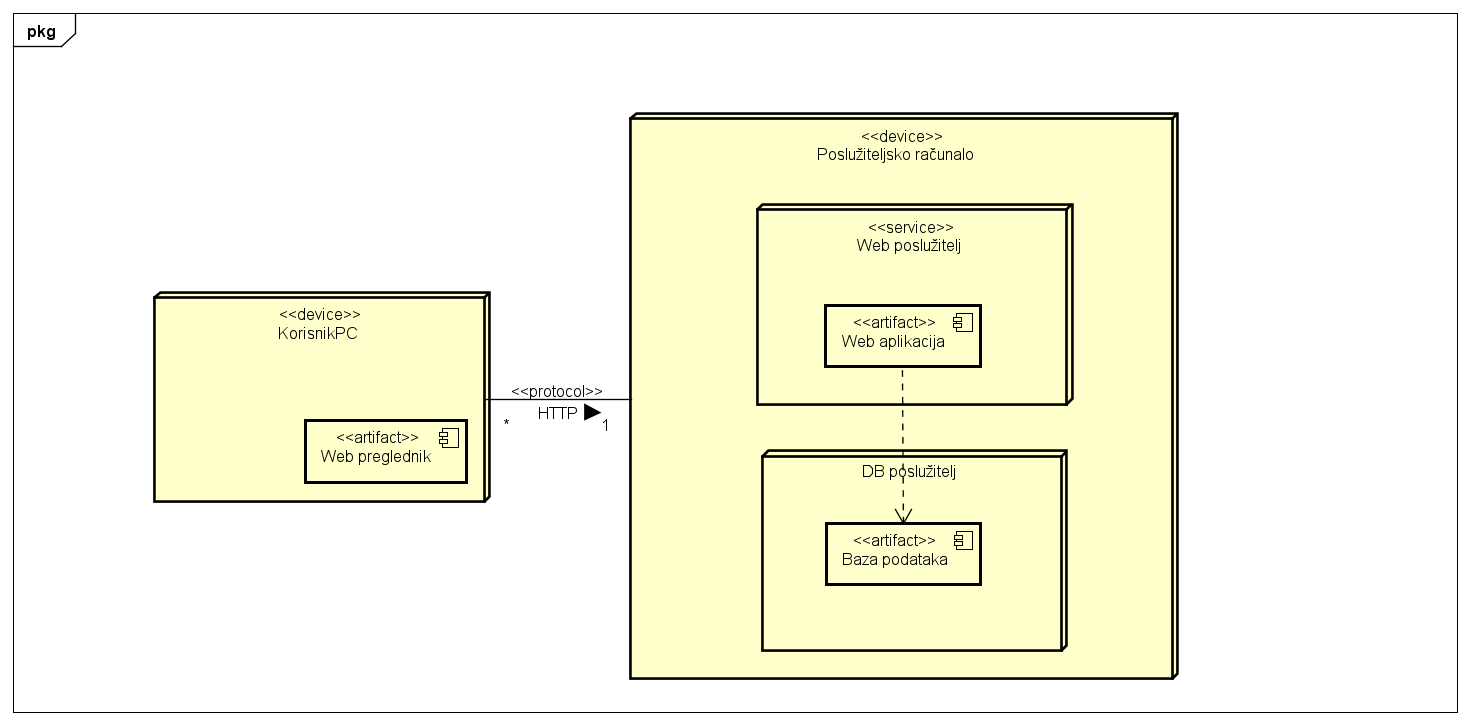
\includegraphics[scale=0.5]{slike/dijagram_razmjestaja.png} %veličina slike u odnosu na originalnu datoteku i pozicija slike
				\centering
				\caption{Dijagram razmještaja}
				\label{fig:promjene}
			\end{figure}
			
			\eject 
		
		\section{Upute za puštanje u pogon}
		
			\textbf{\textit{dio 2. revizije}}\\
		
			 \textit{U ovom poglavlju potrebno je dati upute za puštanje u pogon (engl. deployment) ostvarene aplikacije. Na primjer, za web aplikacije, opisati postupak kojim se od izvornog kôda dolazi do potpuno postavljene baze podataka i poslužitelja koji odgovara na upite korisnika. Za mobilnu aplikaciju, postupak kojim se aplikacija izgradi, te postavi na neku od trgovina. Za stolnu (engl. desktop) aplikaciju, postupak kojim se aplikacija instalira na računalo. Ukoliko mobilne i stolne aplikacije komuniciraju s poslužiteljem i/ili bazom podataka, opisati i postupak njihovog postavljanja. Pri izradi uputa preporučuje se \textbf{naglasiti korake instalacije uporabom natuknica} te koristiti što je više moguće \textbf{slike ekrana} (engl. screenshots) kako bi upute bile jasne i jednostavne za slijediti.}
			
			
			 \textit{Dovršenu aplikaciju potrebno je pokrenuti na javno dostupnom poslužitelju. Studentima se preporuča korištenje neke od sljedećih besplatnih usluga: \href{https://aws.amazon.com/}{Amazon AWS}, \href{https://azure.microsoft.com/en-us/}{Microsoft Azure} ili \href{https://www.heroku.com/}{Heroku}. Mobilne aplikacije trebaju biti objavljene na F-Droid, Google Play ili Amazon App trgovini.}
			 
			Za puštanje u korištena je WEB usluga Render istoimene tvrtke, te se puštanje u pogon treba obaviti prema zahtjevima Render platforme. 
			 	
			 \textbf{Stvaranje Render korisničkog računa}
			 	
			 \textbf{Konfiguracija baze podataka na Renderu}
			 
			 Na Renderu je potrebno napraviti novu Postgres bazu podataka odabirom opcije new na Renderovoj radnoj traci. Potom se odabire opcija PostgreSQL. Potrebno je popuniti sva polja poput imena baze, imena korisnika...
			 
			 \textbf{Odabir regije i verzije PostgreSQL-a}
			 
			 Na korsiničkom sučelju potrebno je odabrati verziju PostgreSQL-a koja će se koristiti i regiju poslužitelja s kojeg će Render posluživati korisnike. Render će generirati URL baze podataka koji će biti potrebni za daljnje korake puštanja u pogon.
			 
			 \textbf{Stvaranje backend poslužitelja}
			 
			 Unutar Rendera odaberemo opciju new WEB usluga, te odaberemo opciju "Build and deploy from git repository." Nakon toga sljedi proces povezivanja GitHub korisničkog računa i repozitorija s Render korisničkim računom.
			 
			 Upiši ime servisa i regiju
			 
			 Odaberi branch repo koji se deploya
			 
			 Postavi root direktorij za aplikaciju
			 
			 Odaberi runntime okolinu odaberi docker 
			 
			 Proširi advanced postavke 
			 
			 Dodaj potrebne varijable okoline poput imena baze, šifre baze i URL baze. Pozornost na format baze.
			 
			 Putanja docker file-a
			 
			 TO JE BACKEND
			 
			 Frontend 
			 
			 U package.json dodaj sve dependencie za deploy
			 
			 U package.json build zamjeni build s ovim sto treba
			 
			 Dodaj ono sta je onom sto ce ti Dominik poslat
			 
			 Na render dashboard new webservice povezi git bla bla bla
			 
			 Nakon region ce ic build command postavi na yarn build a start commandu da start-prod. 
			 
			 Proširi advanced i enviroment var dodat adresu deployanog backenda i klikunut create web service
			 
			 
			 
			 
			 	
			 		
			
			
			\eject 